\documentclass[11pt,spanish,a4paper]{article}
% Versión 1.er cuat 2021 Víctor Bettachini < bettachini@df.uba.ar >

% Versión 1.er cuat 2021 Víctor Bettachini < bettachini@df.uba.ar >

\usepackage[T1]{fontenc}
\usepackage[utf8]{inputenc}

\usepackage[spanish, es-tabla]{babel}
\def\spanishoptions{argentina} % Was macht dass?
% \usepackage{babelbib}
% \selectbiblanguage{spanish}
% \addto\shorthandsspanish{\spanishdeactivate{~<>}}

\usepackage{graphicx}
\graphicspath{{./figuras/}}
% \usepackage{float}

\usepackage[arrowdel]{physics}
\newcommand{\pvec}[1]{\vec{#1}\mkern2mu\vphantom{#1}}
% \usepackage{units}
\usepackage[separate-uncertainty=true, multi-part-units=single, locale=FR]{siunitx}
\usepackage{isotope} % $\isotope[A][Z]{X}\to\isotope[A-4][Z-2]{Y}+\isotope[4][2]{\alpha}

\usepackage{tasks}
\usepackage[inline]{enumitem}
% \usepackage{enumerate}

\usepackage{hyperref}

% \usepackage{amsmath}
% \usepackage{amstext}
\usepackage{amssymb}

\usepackage{tikz}
\usepackage{tikz-dimline}
\usetikzlibrary{math}
\usetikzlibrary{arrows.meta}
% \usetikzlibrary{snakes}
% \usetikzlibrary{calc}
\usetikzlibrary{decorations.pathmorphing}
\usetikzlibrary{patterns}

\usepackage[hmargin=1cm,vmargin=1.6cm,nohead]{geometry}
% \voffset-3.5cm
% \hoffset-3cm
% \setlength{\textwidth}{17.5cm}
% \setlength{\textheight}{27cm}

\usepackage{lastpage}
\usepackage{fancyhdr}
\pagestyle{fancyplain}
\fancyhead{}
\fancyfoot{{\tiny \textcopyright DF, FCEyN, UBA}}
\fancyfoot[C]{ {\tiny Actualizado al \today} }
\fancyfoot[RO, LE]{Pág. \thepage/\pageref{LastPage}}
\renewcommand{\headrulewidth}{0pt}
\renewcommand{\footrulewidth}{0pt}


\begin{document}
\begin{center}
\textbf{Física 2} (Físicos) \hfill \textcopyright {\tt DF, FCEyN, UBA}\\
	\textsc{\LARGE Ondas viajeras y estacionarias}
\end{center}


Los ejercicios con (*) entrañan una dificultad adicional. Son para investigar después de resolver los demás.



\begin{enumerate}


\input{\detokenize{parámetrosPropagantes}}

\section*{Estacionaria en una cuerda como superposición de propagantes}

\item 
\begin{minipage}[t][2cm]{0.6\textwidth}
Una cuerda de longitud $L = \SI{0.6}{\metre}$, fija en sus dos extremos, oscila en uno de sus modos normales.
La velocidad de propagación de las ondas en dicha cuerda es \(v = \SI{80}{\metre\over\second}\).
En el momento que presenta su máxima amplitud pico a pico ésta es de \SI{8}{\milli\metre}.
\end{minipage}
\begin{minipage}[c][1.5cm][t]{0.34\textwidth}
	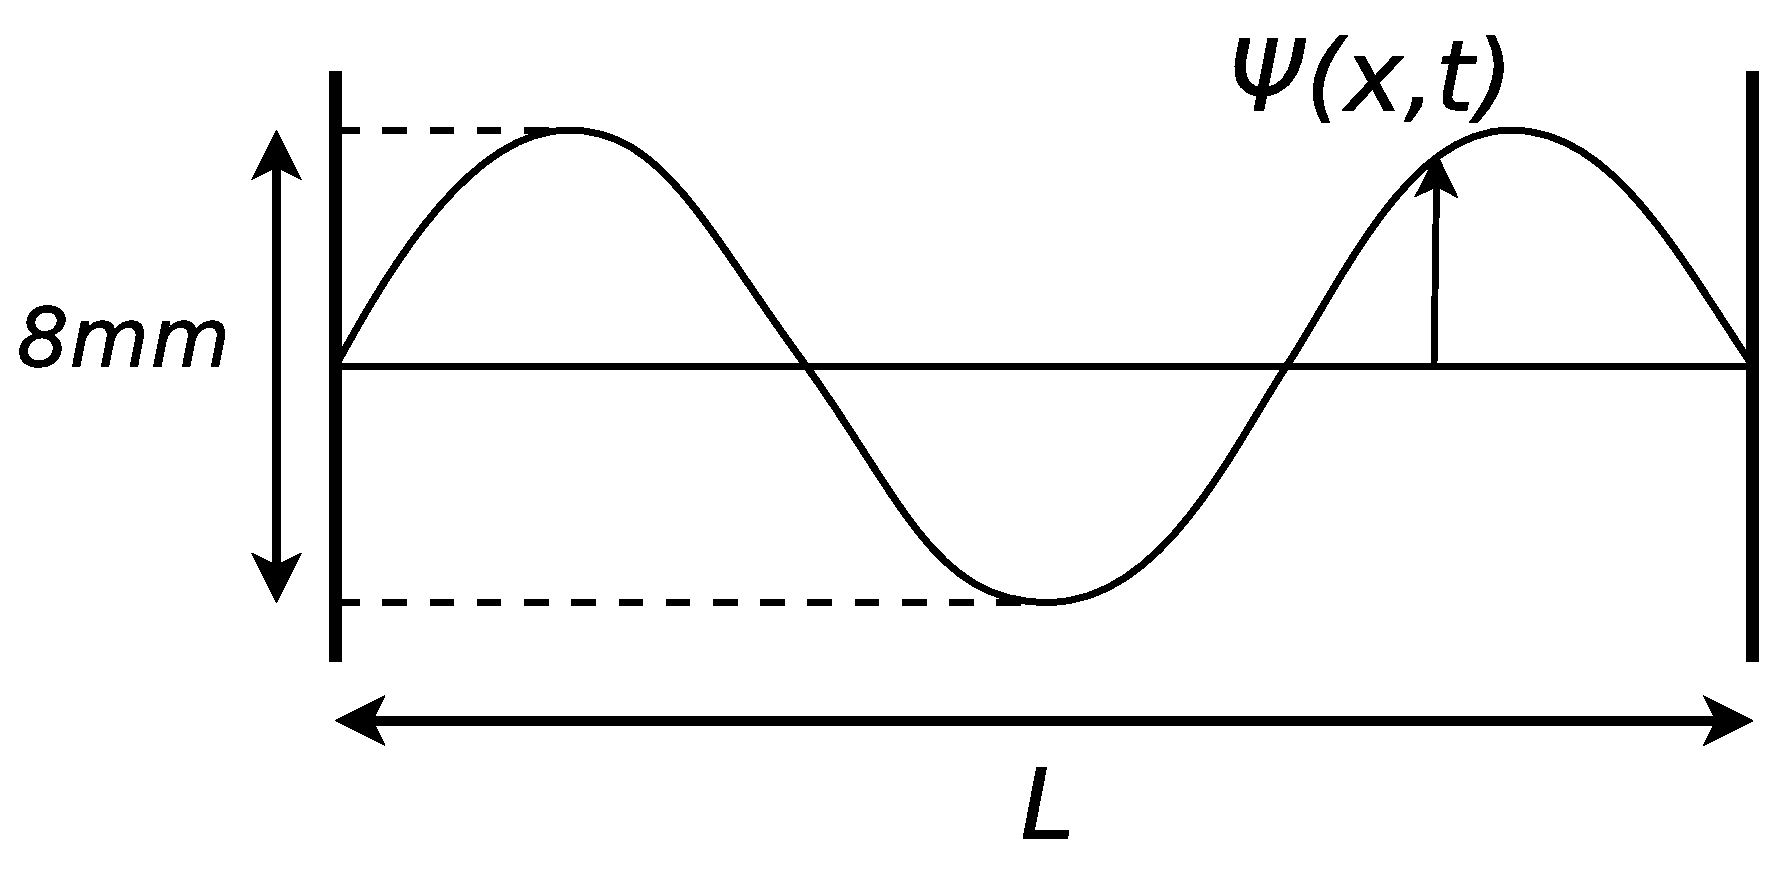
\includegraphics[width=\textwidth]{ej1-32}
\end{minipage}
\begin{enumerate}
	\item Escribir $\Psi(x,t)$, sabiendo que $\Psi(x,0) = 0\;\forall x$, y que $\dot{\Psi}(L/2,0) > 0$.
	\item Hallar las ondas propagantes $\Psi_{1,2}$ tales que $\Psi(x,t)$ sea una combinación lineal de éstas.
\end{enumerate}


\item 
\begin{minipage}[t][2.6cm]{0.6\textwidth}
Una cuerda de longitud $L = \SI{1}{\metre}$, con un extremo fijo y uno libre, oscila en uno de sus modos normales.
La velocidad de propagación de las ondas en dicha cuerda es \(v= \SI{80}{\metre\over\second}\).
En \(t = 0\) presenta su máxima amplitud pico a pico de \SI{8}{\milli\metre}, siendo $\Psi(L,0) > 0$.
\end{minipage}
\begin{minipage}[c][0.4cm][t]{0.34\textwidth}
	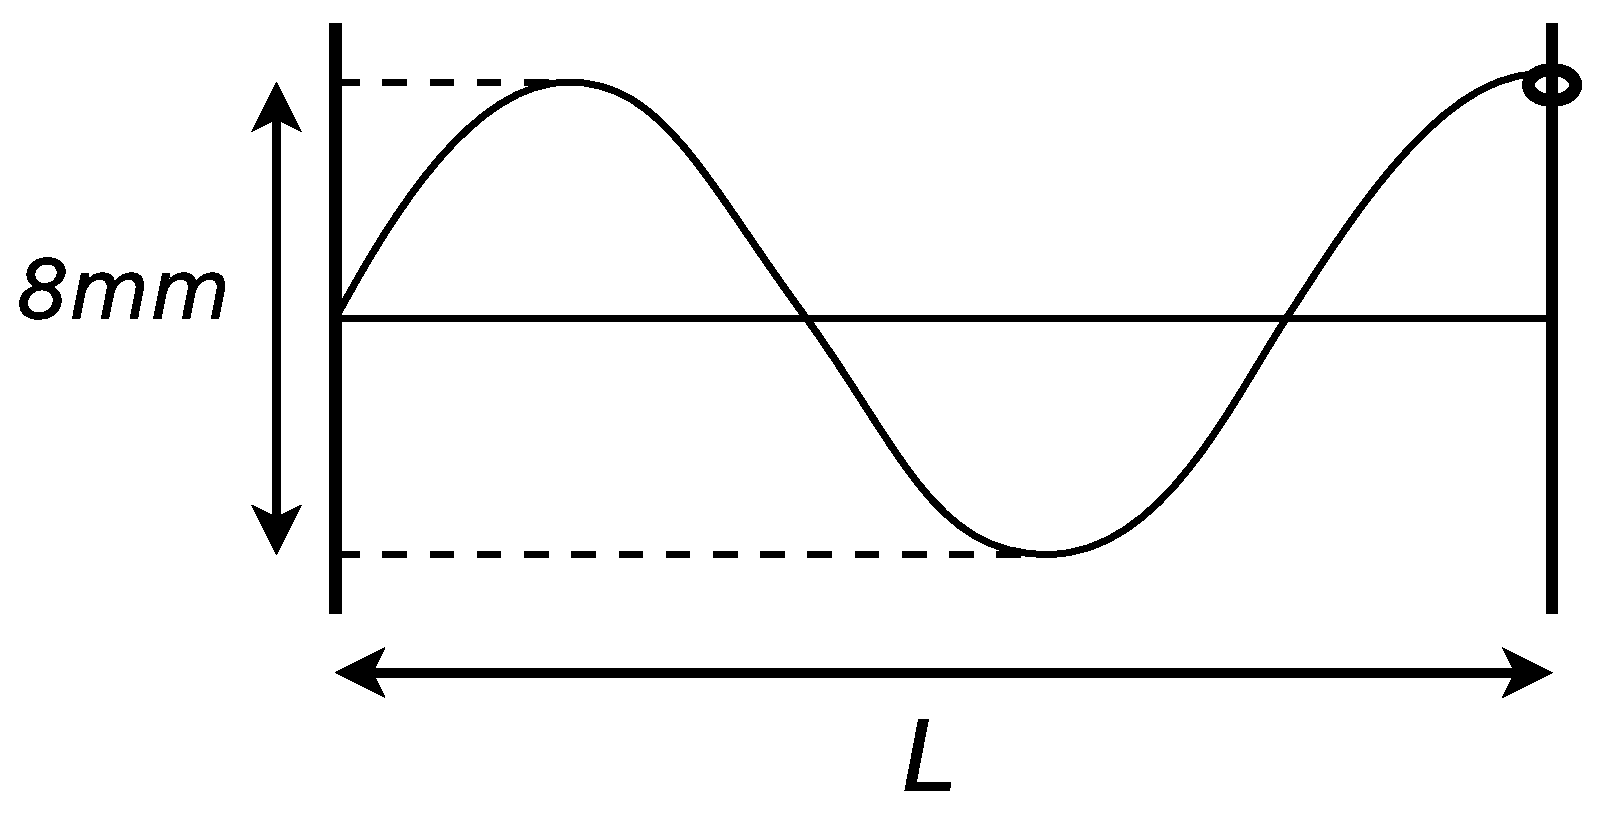
\includegraphics[width=\textwidth]{ej1-33}
\end{minipage}
\begin{enumerate}
	\item Resolver, para esta situación, todo lo pedido en el problema anterior. 
	\item Si ahora la cuerda está oscilando en un modo normal arbitrario $n$, con las mismas condiciones iniciales dadas arriba, repetir (a) (expresar en función de $n$).
\end{enumerate}



\end{enumerate}

\end{document}
